\section{Null model construction}\label{sec:nullmodel}
The kind of data considered in this work comes from RNA Sequencing experiments. These experiments use wet biology methods to extract information from samples. If one imagines it exists an unknown function that describes the gene expression across the samples considered, what experimental people do is to sample this function, picking up some genes.

In this section it is described a null model of sampling, this is useful to verify if the data distributions seen are just an effect of this experimental sample or if they carry some useful and interesting information.

As described in~\cite{Mazzolini2018}, a random matrix has to be created. This matrix is a collection of components and realizations exactly as~\ref{fig:componetstable}. The values of each component abundances in each realization $n_{i j}$ are randomly assigned with a probability determined by 
the global abundance in the whole dataset~\ref{eq:abundance}. Values of each column are extracted until the size~\ref{eq:size} is 
reached. Strictly speaking it is a multinomial process with probability
\begin{equation}
P\left( \{ n_i\} ;M\right) =\frac{M!}{\prod_{i=1}^{N} n_i}\prod_{i=1}^N f_i^{n_i}
\end{equation}
where $n_i$ is the number of times the component with frequency $f_i$ appears, being $f_i=\frac{a_i}{\sum_{c=1}^{N}a_{c}}$ as defined in~\ref{eq:fi}.

Figure~\ref{fig:structure/randomsampling} shows an example of this, $M$ components are picked up concerning their frequency in the dataset. The most abundant components, which are also the ones with the highest frequencies (frequency is nothing but the normalized abundance), have a greater probability to be picked up.
\begin{figure}[htb!]
    \centering
    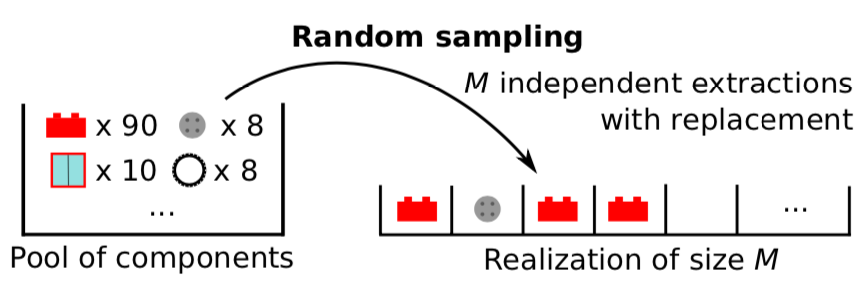
\includegraphics[width=0.8\linewidth]{pictures/structure/randomsampling.png}
    \caption{Random sampling of components to build a realization of size $M$.}
    \label{fig:structure/randomsampling}
\end{figure}

Using this construction on real counts data, by definition the Zipf's law sampled is identical to the data's one.
\begin{figure}[htb!]
\begin{minipage}{0.5\textwidth}
    \centering
    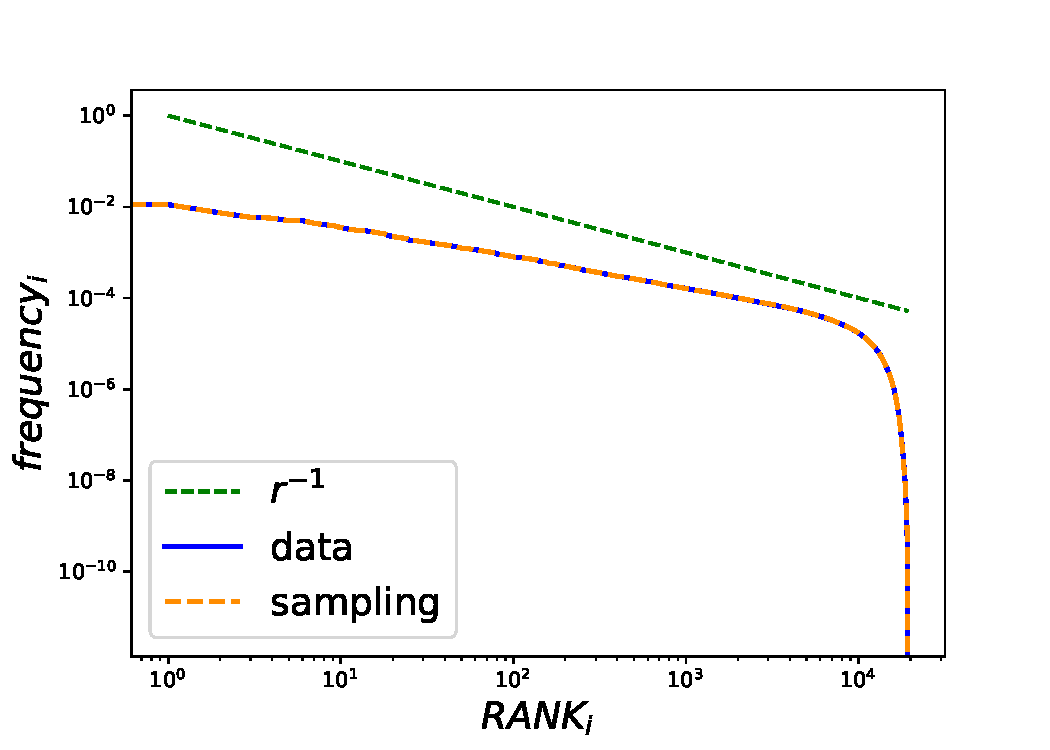
\includegraphics[width=0.95\linewidth]{pictures/structure/tcga/globalzipf_null.pdf}
\end{minipage}
\hspace{2mm}
\begin{minipage}{0.5\textwidth}
    \centering
    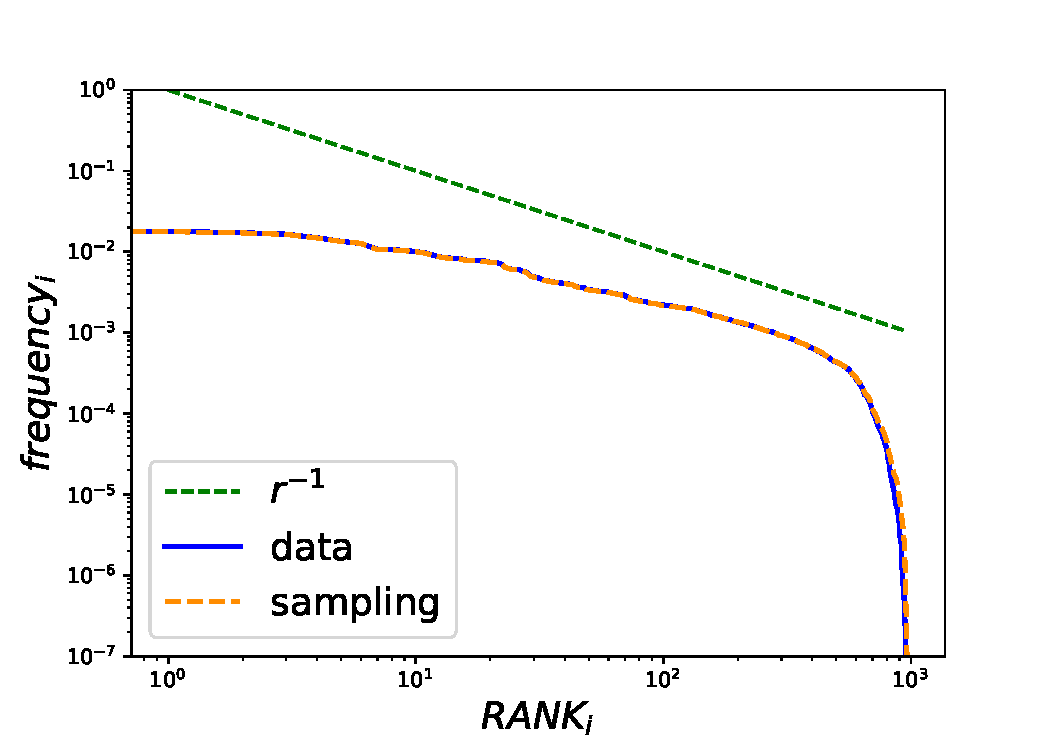
\includegraphics[width=0.95\linewidth]{pictures/structure/gtex/globalzipf_null.pdf}
\end{minipage}
\caption{Zipf's law sampled; TCGA(left) and GTEx (right). By definition original frequencies and sampled ones are identical.}
\label{fig:structure/globalzipf_null}
\end{figure}
By construction, the distribution of the sizes of the sampling and the data are also identical.
\begin{figure}[htb!]
\begin{minipage}{0.5\textwidth}
    \centering
    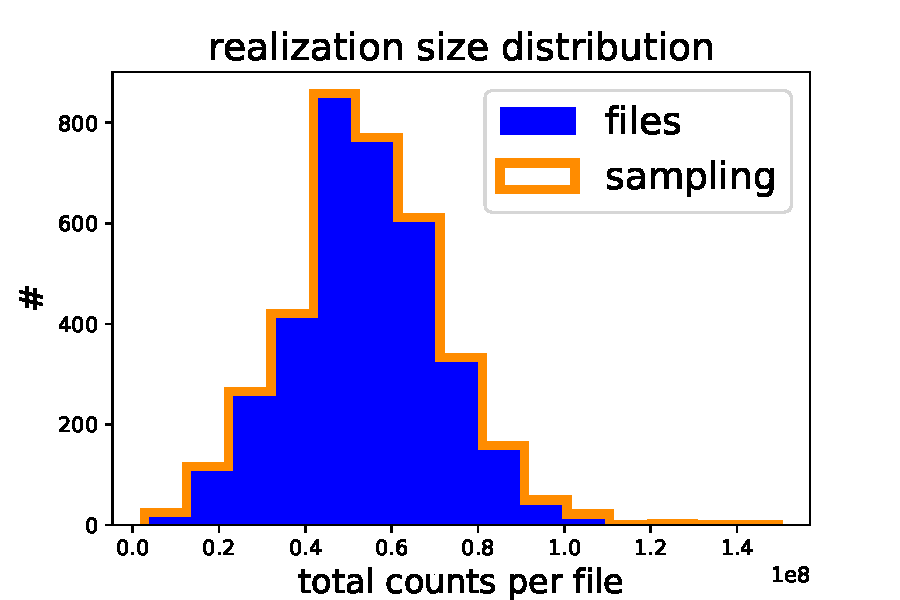
\includegraphics[width=0.95\linewidth]{pictures/structure/tcga/sizeDistr_null.pdf}
\end{minipage}
\hspace{2mm}
\begin{minipage}{0.5\textwidth}
    \centering
    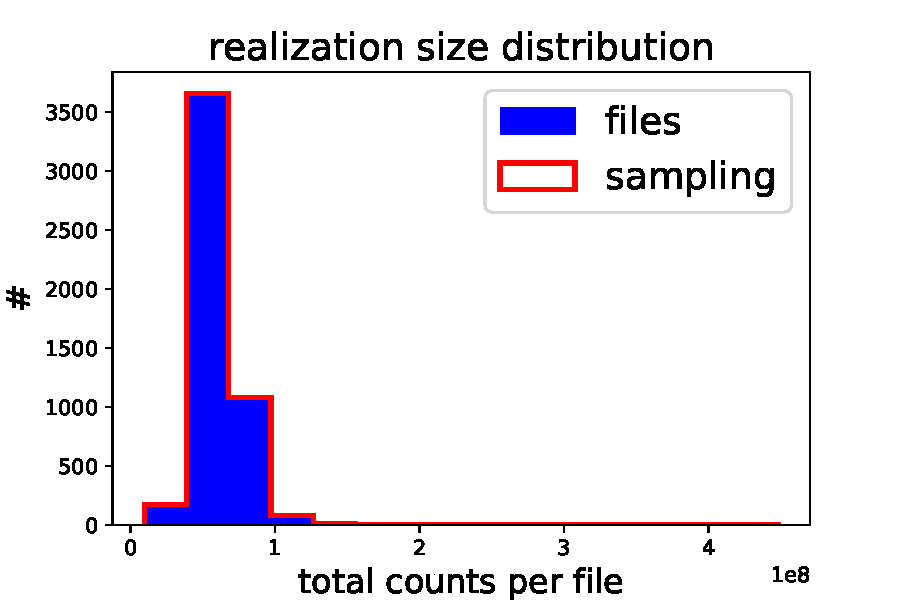
\includegraphics[width=0.95\linewidth]{pictures/structure/gtex/sizeDistr_null.pdf}
    \end{minipage}
\caption{Distribution of sizes $M$; TCGA(left) and GTEx (right). By definition sampling and original sizes are identical.}
    \label{fig:structure/sizeDistr_null}
\end{figure}

Looking at the $U$s in figure~\ref{fig:structure/globalU_null}, it is evident that data behave differently from sampling. This is a signal that the null model is not enough to explain the data matrices. In particular, it is evident that the null model generates the matrices in a manner such that more components have high occurrence comparing to the original data. This can be easily explained, in fact in the real world some genes are highly expressed but only in a subset of the whole dataset; these genes are specific for certain type of samples. The null model gets the information that such genes are highly expressed (they have a high abundance) and so samples these quite often (components with high abundance have a greater chance to be picked up by the null model sampling). This set of genes with $O_i=1$ is called \textbf{core}, in figure~\ref{fig:structure/globalU_null} it is evident the difference between the real one and the sampled one.
\begin{figure}[htb!]
\begin{minipage}{0.5\textwidth}
    \centering
    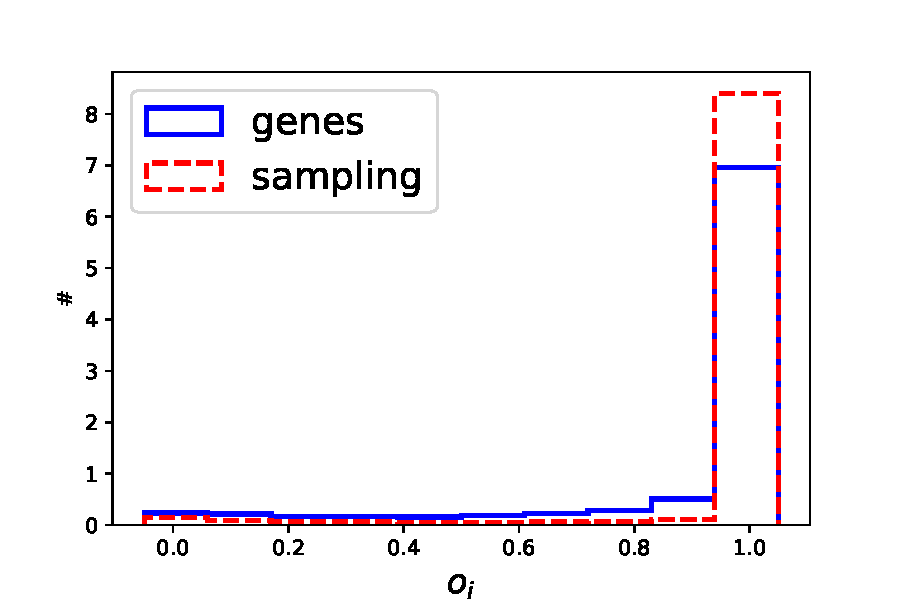
\includegraphics[width=0.95\linewidth]{pictures/structure/tcga/globalU_null.pdf}
\end{minipage}
\hspace{2mm}
\begin{minipage}{0.5\textwidth}
    \centering
    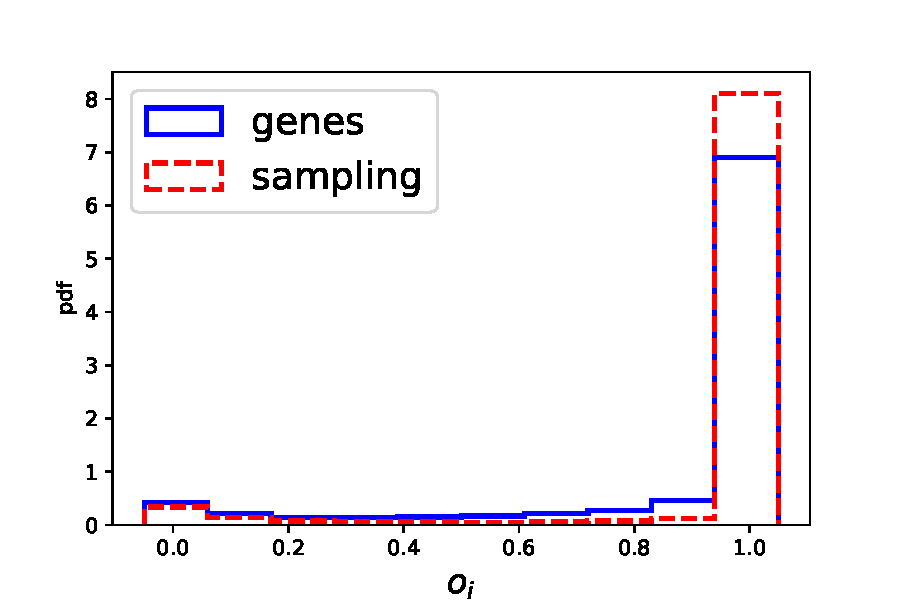
\includegraphics[width=0.95\linewidth]{pictures/structure/gtex/globalU_null.pdf}
    \end{minipage}
\caption{Occurrence distributions; TCGA(left) and GTEx (right). Sampling is reported for comparison.}
\label{fig:structure/globalU_null}
\end{figure}

Plotting on the abscissa the size of samples and on the ordinate the number of genes expressed one point per sample, it is possible to obtain the so-called Heaps's law~\cite{Heaps:1978:IRC:539986}. In figure~\ref{fig:structure/heaps_null} the Heaps' law is presented compared to the one obtained by sampling. Again the curves differ and the null model is not enough to explain the trend. Note that each data point shares the abscissa with a sampling one (figures~\ref{fig:structure/sizeDistr_null} are nothing but the histograms of the abscissas of~\ref{fig:structure/heaps_null}). Moreover, it is interesting that the ordinate does not start from zero, this happens because there are a lot of genes that express everywhere, the core. It happens that the sampling curve is translated above the data's one. This means that to build a sample of size $M$ just by sampling it is necessary to use a greater number of different genes than the number of different genes actually expressed in nature. In other words in the real world only the genes that are really useful in a sample are expressed, and this is not describable just by sampling. This fact is coherent with the fact that the $U$s differ.
\begin{figure}[htb!]
\begin{minipage}{0.5\textwidth}
    \centering
    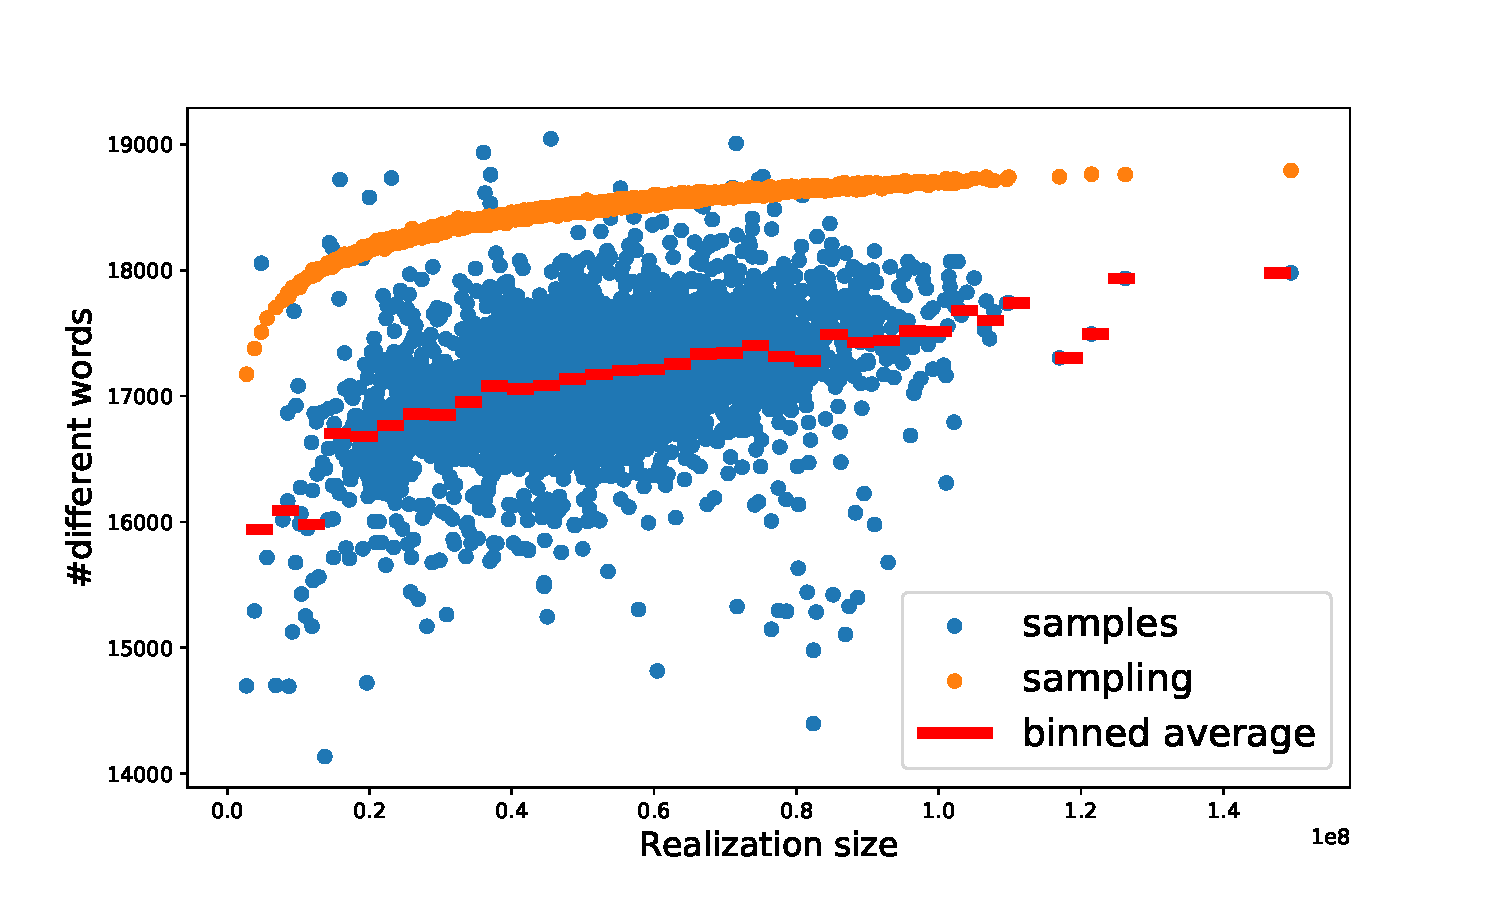
\includegraphics[width=0.95\linewidth]{pictures/structure/tcga/heaps_null.pdf}
    \end{minipage}
\hspace{2mm}
\begin{minipage}{0.5\textwidth}
    \centering
    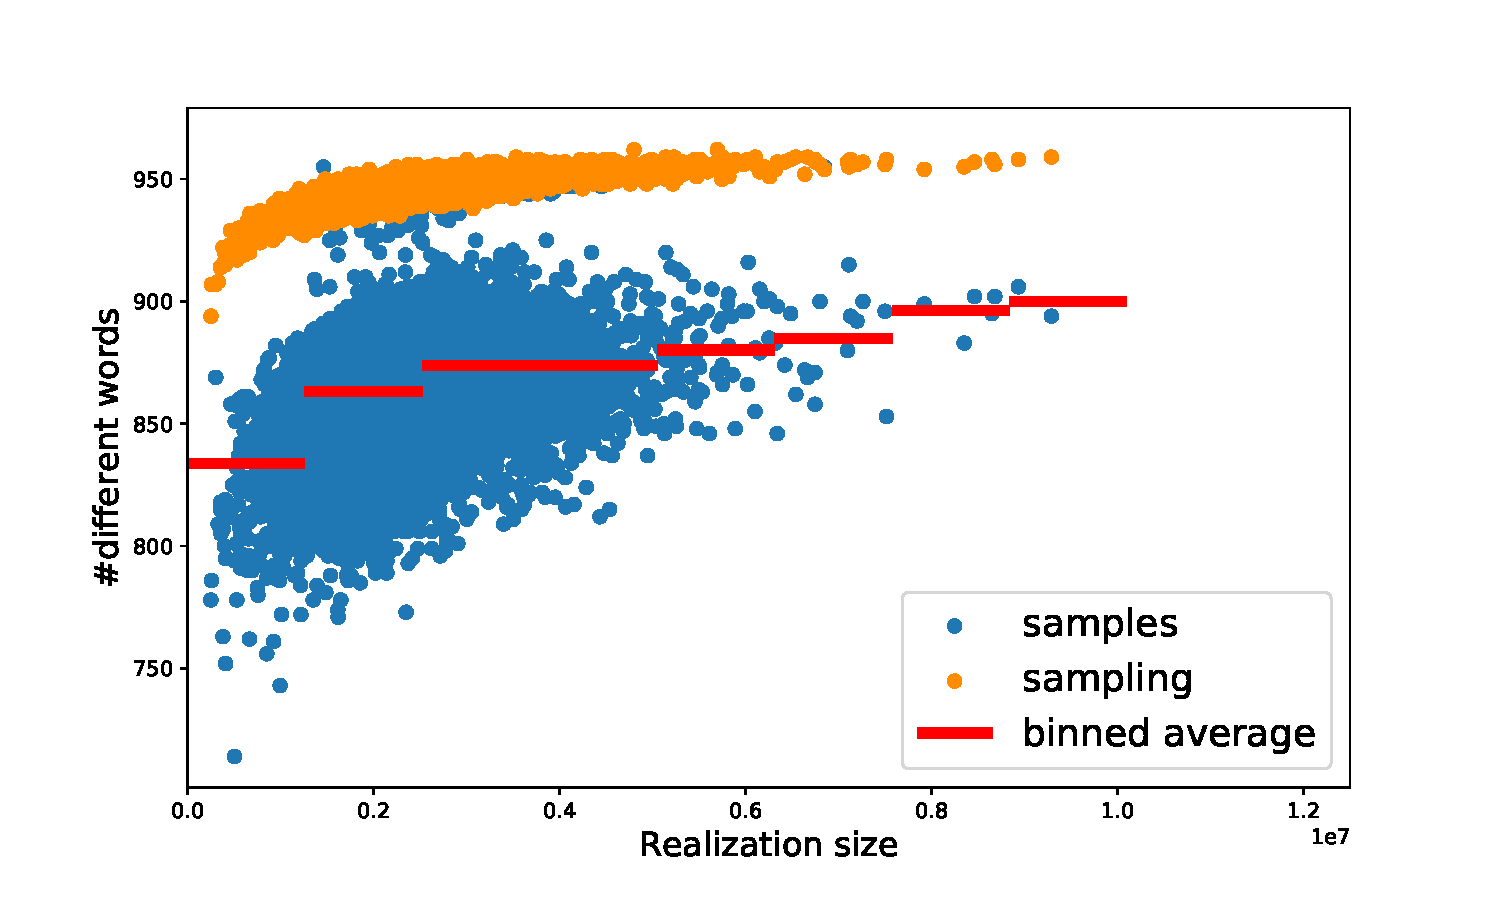
\includegraphics[width=0.95\linewidth]{pictures/structure/gtex/heaps_null.pdf}
    \end{minipage}
\caption{Heaps' law; TCGA(left) and GTEx (right). Sampling is reported for comparison.}
\label{fig:structure/heaps_null}
\end{figure}
Another way to see this is by looking at the histograms of the number of different genes expressed, actually the distribution of the~\ref{fig:structure/heaps_null} y-axis. Figure~\ref{fig:structure/diffwordsDistr_null} shows that these distributions are completely different if one looks at the data and the samples.
\begin{figure}[htb!]
\begin{minipage}{0.5\textwidth}
    \centering
    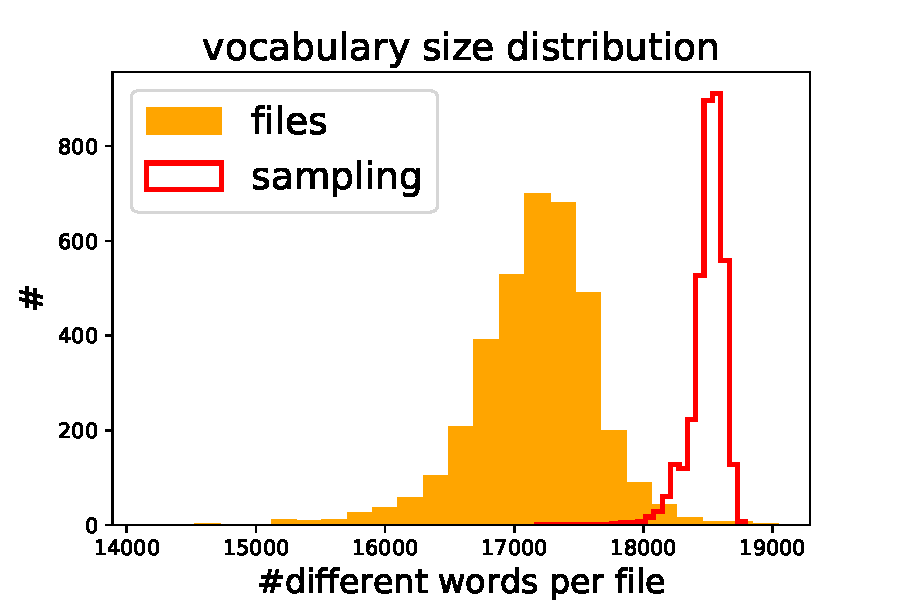
\includegraphics[width=0.95\linewidth]{pictures/structure/tcga/diffwordsDistr_null.pdf}
    \end{minipage}
\hspace{2mm}
\begin{minipage}{0.5\textwidth}
    \centering
    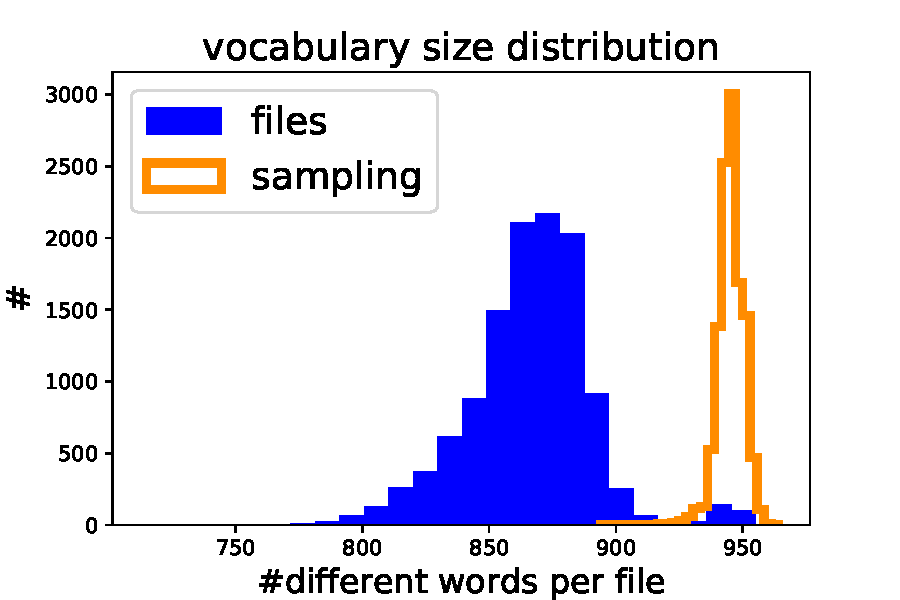
\includegraphics[width=0.95\linewidth]{pictures/structure/gtex/diffwordsDistr_null.pdf}
    \end{minipage}
\caption{Number of genes expressed in a sample; TCGA(left) and GTEx (right). The difference between the original data and sampling is evident.}
\label{fig:structure/diffwordsDistr_null}
\end{figure}